\chapter{Kết quả thực nghiệm}

\textit{Trong chương này, đề tài trình bày các kết quả đạt được sau quá trình thiết kế, tổng hợp và triển khai hệ thống SoC trên nền tảng phần cứng thực tế. Nội dung bao gồm đánh giá tài nguyên sử dụng, kết quả kiểm tra các khối ngoại vi, hiệu năng của Video Streaming và quy trình khởi động hệ thống thông qua Bootloader.}

\section{Môi trường thực nghiệm phần cứng}

Toàn bộ hệ thống SoC được triển khai và đánh giá trên kit phát triển \textbf{Xilinx Virtex-7 VC707 FPGA} và  \textbf{Arty A7-100T Artix-7 FPGA}. Các FPGA này đều cung cấp đầy đủ các giao diện cần thiết cho việc thực nghiệm.

Các thông số thiết lập xung nhịp hệ thống bao gồm:
\begin{itemize}
    \item[] Xung nhịp hệ thống chính (\texttt{sys\_clk}): 200 MHz đối với VC707 và 100 MHz đối với Arty A7.
    \item[] Xung nhịp chính cho khối Video Streaming là 150 MHz trên VC707, còn Arty A7 không đủ bộ nhớ Bram nên sẽ không triển khai khối Video Streaming trên đây.
    \item[] Xung nhịp hiển thị (\texttt{pixel\_clk}): 25 MHz và 50 MHz.
\end{itemize}

\section{Kết quả hiện thực các khối giao tiếp ngoại vi}

Hệ thống đã hoàn thiện việc tích hợp và kiểm tra độ tin cậy của các chuẩn giao tiếp nối tiếp quan trọng, đảm bảo khả năng tương tác toàn diện với các thiết bị ngoại vi.

\subsection{Giao tiếp UART}
Khối UART đã được thực nghiệm thành công với các tốc độ baud chuẩn như: 9600, 115200, 230400, 460800 bps. Kết quả kiểm tra thông qua phần mềm Terminal (PuTTY) cho thấy dữ liệu được truyền nhận chính xác giữa SoC và máy tính cá nhân, phục vụ tốt cho việc xuất log gỡ lỗi và tương tác lệnh.

\begin{figure}[H]
    \centering
    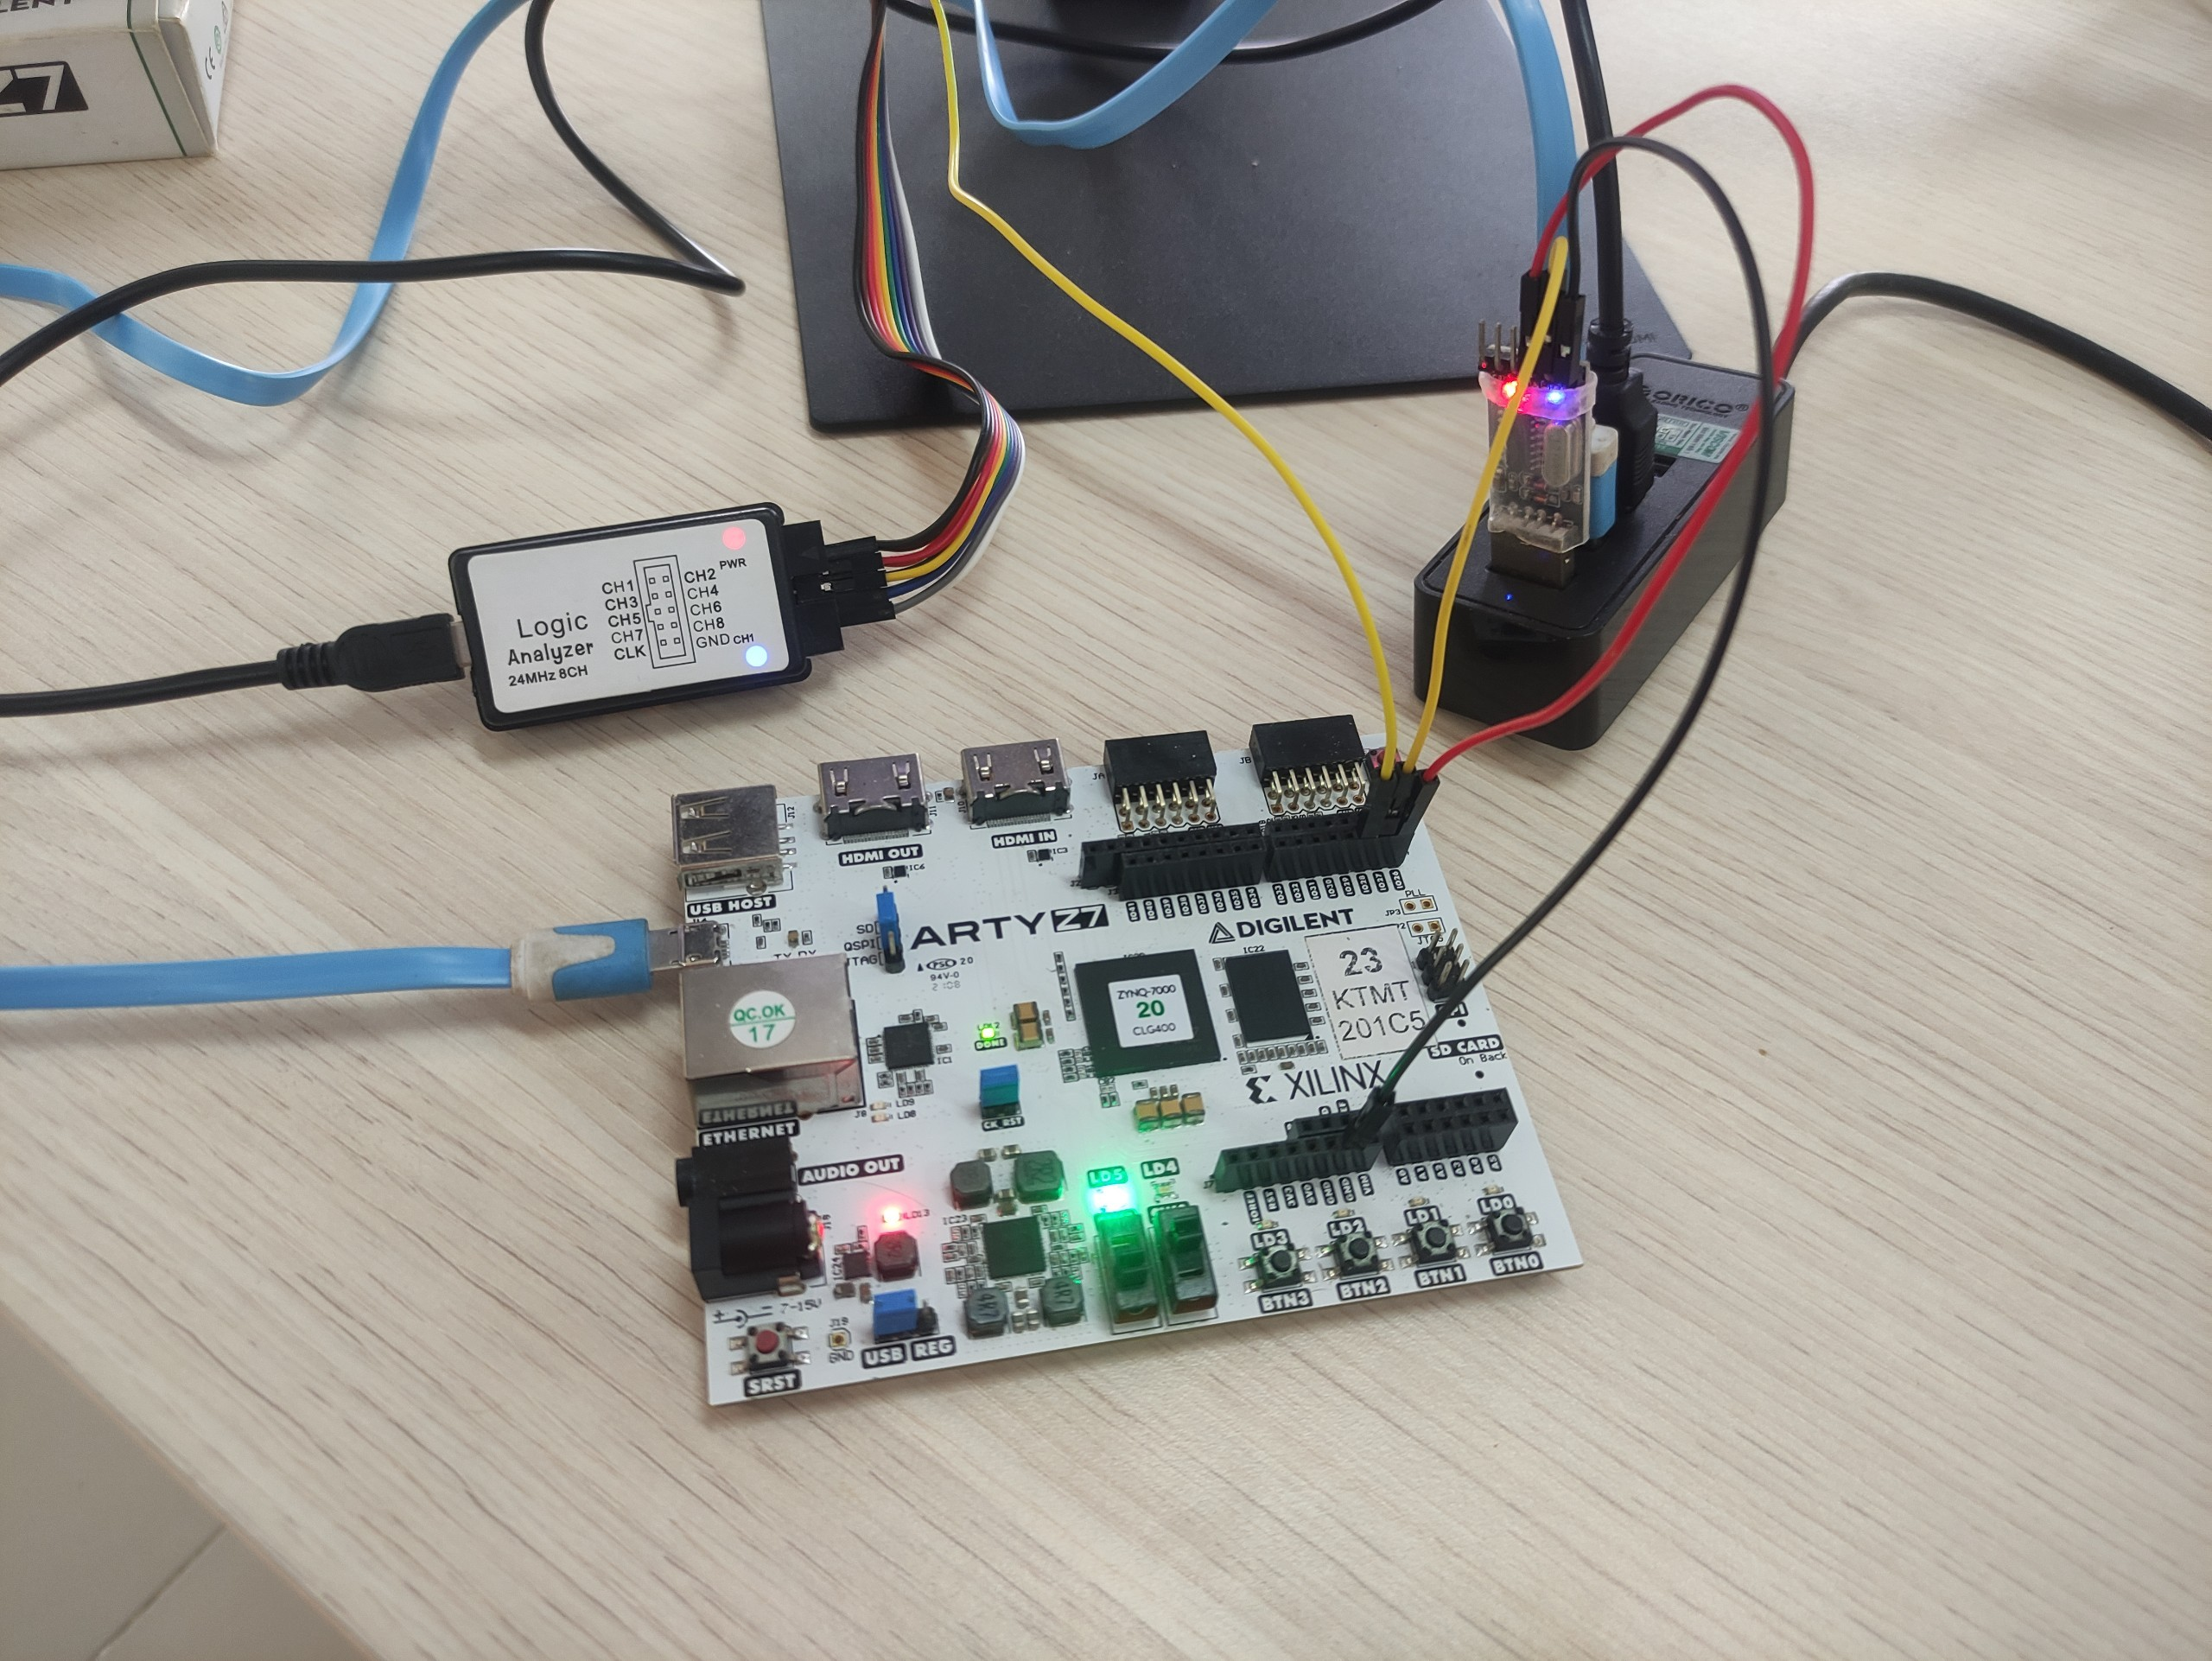
\includegraphics[width=0.9\textwidth]{ket_qua_thuc_nghiem/image/uart.png}
    \caption{Kết nối UART từ Arty A7 với máy tính}
    \label{fig:uart_communication}
\end{figure}

\begin{figure}[H]
    \centering
    \includegraphics[width=0.9\textwidth]{ket_qua_thuc_nghiem/image/uart1.png}
    \caption{Chương trình kiểm thử giao tiếp UART}
    \label{fig:uart_communication}
\end{figure}

\begin{figure}[H]
    \centering
    \includegraphics[width=0.9\textwidth]{ket_qua_thuc_nghiem/image/uart2.png}
    \caption{Cài đặt thông số PuTTY để giao tiếp UART}
    \label{fig:uart_communication}
\end{figure}

\begin{figure}[H]
    \centering
    \includegraphics[width=0.9\textwidth]{ket_qua_thuc_nghiem/image/uart3.png}
    \caption{Kết quả giao tiếp UART thành công}
    \label{fig:uart_communication}
\end{figure}



\subsection{Giao tiếp I2C và SPI}

\textbf{I2C:} Được sử dụng để cấu hình các thanh ghi nội của cảm biến hình ảnh OV5640 và chip phát HDMI ADV7513. Thực nghiệm cho thấy quá trình cấu hình diễn ra ổn định, các thiết bị phản hồi đúng địa chỉ và mã lệnh. \\

\textbf{SPI:} Đã hiện thực hóa bộ điều khiển SPI Master để giao tiếp với bộ nhớ Flash. Thực nghiệm với chip Flash W25Q32 cho kết quả đọc/ghi dữ liệu chính xác ở tốc độ lên đến 25 MHz.   

\begin{figure}[H]
    \centering
    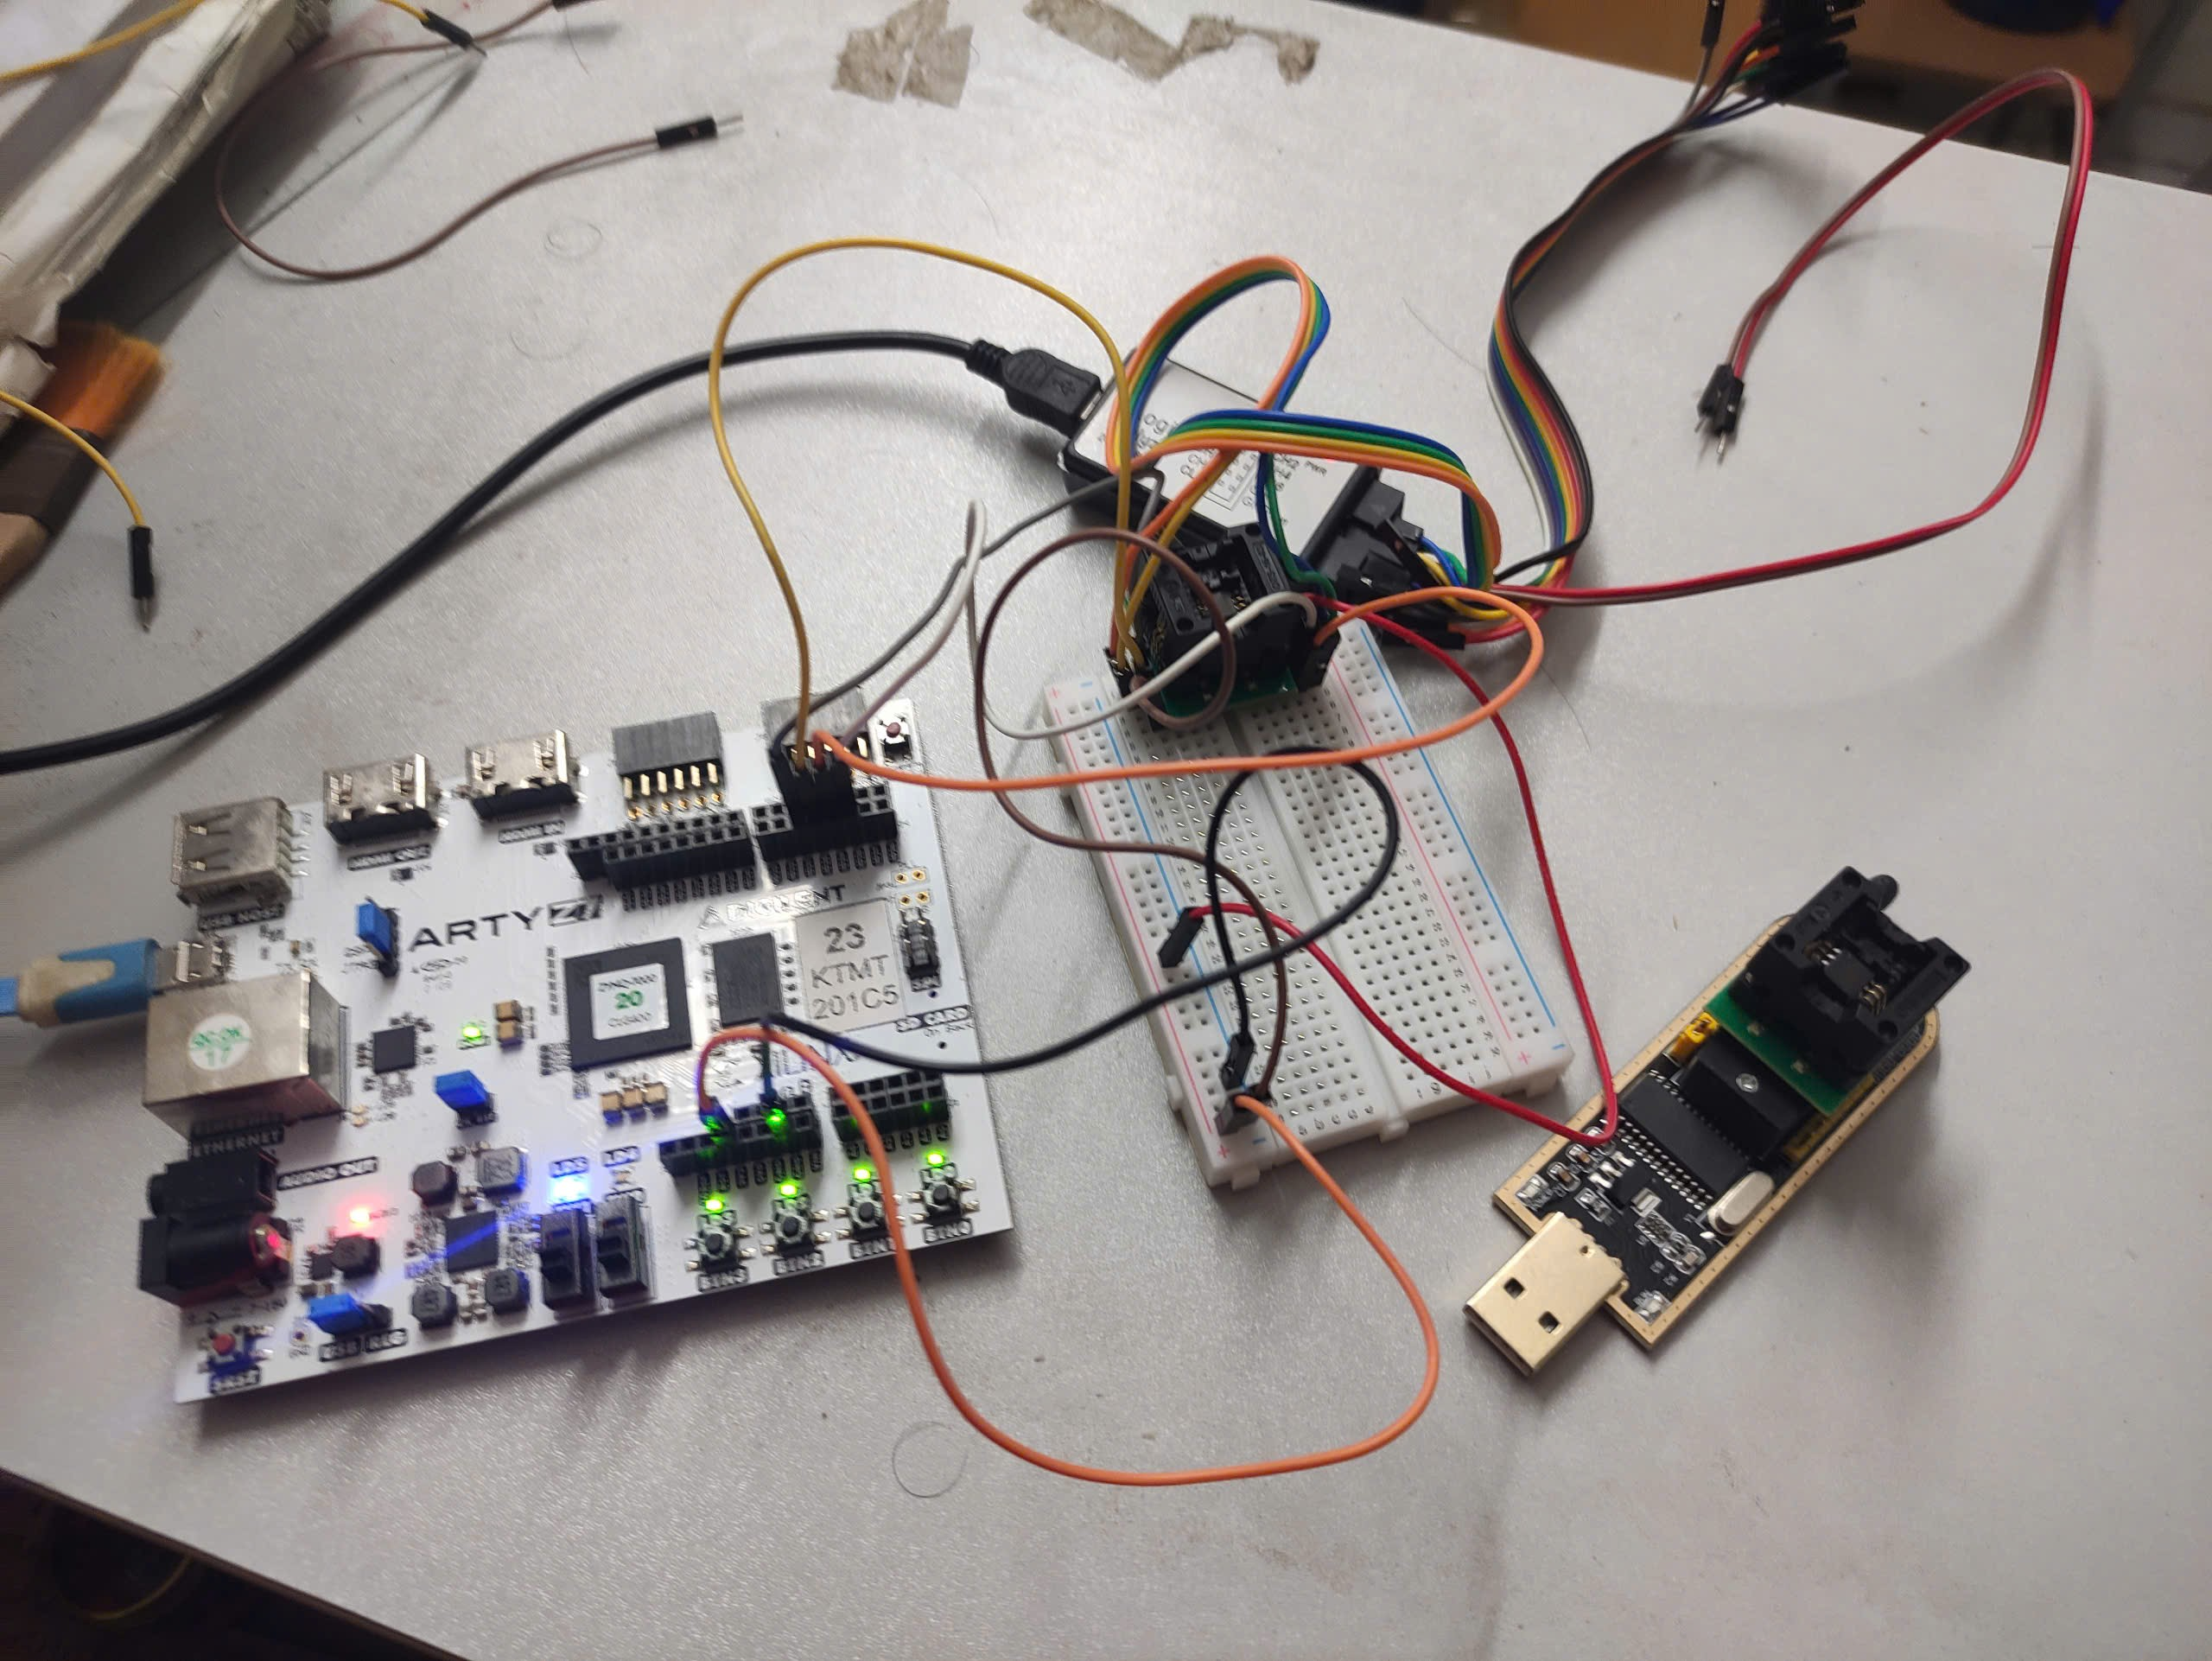
\includegraphics[width=0.9\textwidth]{ket_qua_thuc_nghiem/image/spi.png}
    \caption{Kết nối SPI từ Arty A7 với bộ nhớ Flash}
    \label{fig:spi_communication}
\end{figure}

\begin{figure}[H]
    \centering
    \includegraphics[width=0.9\textwidth]{ket_qua_thuc_nghiem/image/spi1.png}
    \caption{Sơ đồ sóng được đo thực tế bằng Logic Analyzer giữa SPI từ Arty A7 với bộ nhớ Flash}
    \label{fig:spi_communication}
\end{figure}

\subsection{Giao tiếp Octal-SPI (OSPI) hỗ trợ DDR}
Khối OSPI đã được thực nghiệm trực tiếp với chip nhớ \textbf{W958D8NBYA} HyperRAM với dung lượng \textbf{256 Mb}. Tốc độ đạt được là 50MHz trong chế độ DDR, kiểm tra bằng cách ghi dữ liệu vào chip và đọc lại rồi gửi qua Terminal UART để xác nhận tính chính xác của dữ liệu.

\begin{figure}[H]
    \centering
    \includegraphics[width=0.9\textwidth]{ket_qua_thuc_nghiem/image/ospi.png}
    \caption{Kết nối chip nhớ HyperRAM (màu xanh lá) với Arty A7 qua giao tiếp OSPI}
    \label{fig:ospi_communication}
\end{figure}


\begin{figure}[H]
    \centering
    \includegraphics[width=0.9\textwidth]{ket_qua_thuc_nghiem/image/ospi2.png}
    \caption{Chương trình cho việc ghi và đọc dữ liệu qua giao tiếp OSPI và xuất ra Terminal UART}
    \label{fig:ospi_communication}
\end{figure}




\section{Kết quả Video Streaming 60Hz}

Một trong những kết quả trọng tâm của đề tài là việc hiện thực hóa luồng dữ liệu Video thời gian thực từ camera ra màn hình.

\begin{itemize}
    \item[] \textbf{Tốc độ khung hình:} Hệ thống đạt mức hiển thị ổn định \textbf{60 Hz}.
    \item[] \textbf{Độ trễ:} Nhờ vào cơ chế quản lý bộ đệm khung hình (Frame Buffer) bằng BRAM, hiện tượng xé hình và trễ tích lũy đã được triệt tiêu đáng kể.
    \item[] \textbf{Chất lượng hình ảnh:} Tín hiệu xuất ra qua cổng HDMI rõ nét, không có điểm ảnh lỗi, nhưng vẫn còn hai lỗi cần khắc phục, lỗi hình ảnh chạy sang bên phải và lỗi khung hình chưa được đồng bộ với màn hình.
\end{itemize}

\begin{figure}[H]
    \centering
    \includegraphics[width=0.9\textwidth]{ket_qua_thuc_nghiem/image/video.png}
    \caption{Phần cứng Video Streaming trên VC707 hiển thị hình ảnh từ camera OV5640 ra màn hình qua cổng HDMI}
    \label{fig:video_streaming}
\end{figure}

\begin{figure}[H]
    \centering
    \includegraphics[width=0.9\textwidth]{ket_qua_thuc_nghiem/image/video1.png}
    \caption{Kiểm tra Màn hình HDMI ổn định với tần số 60Hz}
    \label{fig:video_streaming}
\end{figure}



\begin{figure}[H]
    \centering
    \includegraphics[width=0.9\textwidth]{ket_qua_thuc_nghiem/image/video3.png}
    \caption{Kiểm tra Patten Bar từ camera OV5640 hiển thị qua HDMI}
    \label{fig:video_streaming}
\end{figure}

\begin{figure}[H]
    \centering
    \includegraphics[width=0.9\textwidth]{ket_qua_thuc_nghiem/image/video2.png}
    \caption{Chế độ Streaming Video thời gian thực từ camera OV5640 qua HDMI}
    \label{fig:video_streaming}
\end{figure}


\section{Hiện thực chương trình Bootloader qua SPI Flash}

Để tăng tính độc lập cho SoC, chương trình \textbf{Bootloader} đã được thiết kế để nạp từ bộ nhớ SPI Flash ngoại vi.
\begin{itemize}
    \item[] \textbf{Quy trình:} Khi hệ thống khởi động (Power-on Reset), lõi PicoRV32 sẽ thực thi mã lệnh từ vùng nhớ ROM khởi tạo, thực hiện đọc dữ liệu thực thi từ SPI Flash và nạp vào bộ nhớ lệnh (IMEM).
    \item[] \textbf{Kết quả:} Hệ thống có khả năng tự khởi động và chạy các ứng dụng phần mềm mà không cần tổng hợp lại trên FPGA.
\end{itemize}

\section{Đánh giá tài nguyên sử dụng trên FPGA}

Dựa trên báo cáo tổng hợp từ công cụ Vivado cho thiết kế SoC (chưa có bộ tăng tốc) trên board VC707, tài nguyên hệ thống được sử dụng rất thấp, cho phép mở rộng thêm các bộ gia tốc AI phức tạp trong tương lai:

\begin{figure}[H]
    \centering
    \includegraphics[width=0.9\textwidth]{ket_qua_thuc_nghiem/image/hieunang.png}
    \caption{a. Mức độ sử dụng tài nguyên FPGA riêng phần Video Streaming trên VC707}
    \label{fig:resource_utilization}
\end{figure}

\begin{figure}[H]
    \centering
    \includegraphics[width=0.9\textwidth]{ket_qua_thuc_nghiem/image/hieunang2.png}
    \caption{b. Mức độ sử dụng tài nguyên FPGA riêng phần Video Streaming trên VC707}
    \label{fig:resource_utilization}
\end{figure}


\begin{figure}[H]
    \centering
    \includegraphics[width=0.9\textwidth]{ket_qua_thuc_nghiem/image/hieunang4.png}
    \caption{c. Mức độ sử dụng tài nguyên FPGA riêng phần SoC trên VC707}
    \label{fig:resource_utilization}
\end{figure}

\begin{figure}[H]
    \centering
    \includegraphics[width=0.9\textwidth]{ket_qua_thuc_nghiem/image/hieunang3.png}
    \caption{d. Mức độ sử dụng tài nguyên FPGA riêng phần SoC trên VC707}
    \label{fig:resource_utilization}
\end{figure}

Việc chỉ sử dụng 15\% BRAM trong khi vẫn duy trì được luồng Video 60Hz và đầy đủ các ngoại vi cho thấy hiệu quả cao của kiến trúc quản lý bộ đệm và hệ thống Bus AXI4-Lite đã thiết kế.